% !TEX root = ../notes_template.tex
\chapter{Ecological Teleconnections}\label{chap:Chap9_EOF}

\section{Nonlocal Drivers of Ecological Dynamics}

The most spectacular events in the natural world often arise when different individuals change their behavior simultaneously across a large landscape. In eastern North America, for example, deciduous trees will rapidly change from summer greens to fall colors over the course of several weeks.  These fall colors then indicate the passing of another summer.  Other famous examples include:
\begin{itemize}
    \item Periodical cicadas that emerge in the northeastern US every 13 or 17 years to reproduce and then die, strewing exoskeletons across the east coast of North America; 

    \item Mass coral spawning, where immobile corals across a large seascape synchronously release gametes for broadcast spawning, likely due to shared responses to the timing of moonrise relative to sunset \cite{lin_moonrise_2021};

    \item Lemming outbreaks in Norwegian grasslands that support the survival of juvenile predators in Arctic ecosystems \cite{ims_determinants_2011}.
\end{itemize}
These are all examples of \myindex{spatial synchrony}, where population densities and/or demographics simultaneously undergo some rapid change at geographically distant locations.  Examples such as these have interested naturalists for thousands of years.  They also have important implications for ecosystem function, e.g., for how bears can follow a \textit{red wave} of salmon that spawn at different times across their foraging landscape \cite{deacy_kodiak_2016}.  

These four examples of population synchrony result from many different mechanisms, including synchronous environmental conditions (\index{exogenous synchrony}\textit{exogenous synchrony}) as well as evolutionary pressures to maximize fitness by synchronizing reproductive or other demographic processes (\index{endogeous synchrony}\textit{endogenous synchrony}).  In each case, an ecologist might then seek to describe the spatial scale at which dynamics are synchronized, the spatial and temporal scale over which synchrony is predictable, the relative importance of various endogenous and exogenous drivers, as well as how this synchrony affects community structure and ecosystem function.  

Given the ubiquity and importance of population synchrony, we introduce techniques to describe broad-scale synchrony in biological systems.  To do so, we first introduce a toolkit that is borrowed from physical scientists.  In particular, oceanographers and atmospheric scientists often study processes that are synchronized even at geographically distant locations, (termed atmospheric, oceanographic, or geophysical \textit{teleconnections}).  As we have already discussed, synchrony at geographically distant locations also occurs in ecological systems, and we will use the term \myindex{ecological teleconnections} for these specific types of synchrony.   

\section{Exploratory Factor Analysis and Empirical Orthogonal Functions} \label{sec:Chap9_EOF}

Physical systems often exhibit predictable oscillations that are driven by daily and seasonal cycles of solar radiation (see Fig. \ref{fig:Chap8_stommel_diagram})\footnote{See https://github.com/james-thorson/Spatio-temporal-models-for-ecologists/Chap\_9 for code associated with this chapter.}.  However, they often also have other modes of variation that repeat with different frequencies and are not associated with solar forcing.  In temperate freshwater lakes, for example, an internal layer arises during spring warming that separates warm surface water from denser cold waters below, and gravity favors an outcome where this \myindex{thermocline} occurs at a constant depth across the entire lake.  However, strong winds from summer storms can then push surface waters downwind, such that the thermocline is deeper downwind than upwind.  When the first summer storm passes and winds stop, the thermocline may start rocking back and forth like the surface of the water in a bathtub.  The depth of this thermocline relative to the lake surface then has a periodic oscillation during summer months, with frequency determined by the size and shape of the lake \cite{stevens_estimation_1997}.  On a larger scale, sea surface temperature in the Atlantic Ocean exhibits cyclic variation that typically occurs with two cycles per year \cite{brandt_annual_2016}, while the El Nino-Southern Oscillation (ENSO) results in cyclic variation in sea surface temperature in the equatorial Pacific Ocean occurring every 2--7 years.  In both of these cases, the frequency of physical oscillations arises from the speed at which physical dynamics propagate through ocean waters in relation to the size of physical boundaries.  These endogenous physical cycles can then propagate up to cyclic dynamics in biological systems.  Importantly, these types of oscillation result in localized impacts on physical measurements (e.g., atmospheric/oceanographic temperature and pressure) in areas that are separated by large geographic distances.  For example, the ENSO cycle has characteristic consequences for oceanography and weather both in South America and the Western Pacific island nations.   

Cycles in physical systems such as these have been studied using \myindex{empirical orthogonal functions} (EOF) for over 50 years \cite{grimmer_space-filtering_1963,kidson_eigenvector_1975}.  Early studies would implement EOF by:
\begin{enumerate}
    \item Assembling a complete matrix \(\mathbf{Y}\) of measurements \(y_{s,t}\) for each site \(s\) and time \(t\), e.g., measuring daily sea surface temperature at different oceanographic stations in the Pacific Ocean;

    \item Centering these data for each site, such that the mean across times \(t \in \{ 1, 2, ..., T \}\) of centered matrix \(y^*_{s,t}\) is zero for each location \(s\);

    \item Calculating the \( T \times T \) covariance \(\mathbf{\Sigma} \) in \(y^*_{s,t}\) for each pair of times \(t_1\) and \(t_2\) and assembling a resulting covariance matrix;

    \item Applying principal components analysis to covariance \(\mathbf{\Sigma} \), i.e., computing the eigendecomposition (see Section \ref{sec:Appendix_eigendecomposition}), extracting one or more eigenvectors \(\mathbf{v}_l\) each with length \(T\), and recording these as \textit{modes of variability};
 
    \item For each mode of variability \(\mathbf{v}_l\), calculating the correlation between it and the value \(\mathbf{y}_{s}\) at each location, then recording this map of correlations as the \textit{response map} associated with that mode of variability.
\end{enumerate}
This procedure for calculating an EOF has then resulted in insights about atmospheric and oceanographic teleconnections over the past decades.  In particular, modes of variability are often then correlated with other time-series (e.g., salmon returns in rivers across North America, \cite{mantua_pacific_1997}) to generate and support hypotheses about demographic drivers for highly mobile animals. 

However, this PCA approach to fitting an EOF model has several drawbacks:
\begin{itemize}
    \item[A] \textit{Complete data}:  it requires having no missing entries in data matrix \(\mathbf{Y}\), and it is unclear how to generalize this approach to ecological surveys, e.g., point-count data that follow a random design and are not already gridded;

    \item[B] \textit{Normally distributed data}: calculating a covariance matrix can be statistically inefficient for data that do not follow a normal distribution, e.g., the ``dust-bunny" (i.e., zero-inflated and right-skewed) distribution that is common when sampling species densities in ecological communities \cite{mccune_origin_2015};

    \item[C] \textit{Failure to propagate variance}:  it is unclear how to estimate the total uncertainty resulting from the sequence of computational steps in the algorithm;

    \item[D] \textit{Inability to partition variance}:  similarly, centering the data prior to analysis makes it difficult to compare the importance of EOF modes with the long-term spatial average of the data.   
\end{itemize}
Due to these limitations, we instead present a spatio-temporal model that has similar properties as this conventional EOF analysis \cite{thorson_defining_2020,wikle_dimension-reduced_1999}, which we will call an \textit{EOF-GLLVM} for reasons explained later.  In particular, we specify:

\begin{equation} \label{eq:Chap9_EOF}
\begin{gathered}
  Y_t(s) \sim f( \mu_t(s), \theta ) \\
  g(\mu_t(s)) = \beta_0 + \omega_s + \sum_{l=1}^{n_{factor}} \lambda_{l,t} \epsilon_l(s)
\end{gathered}    
\end{equation}
where \(f\) is a measurement distribution with variance \(\theta\), \(g\) is a link-function, \( \beta_0 \) is an intercept, \( \omega_s \) is long-term average relative at location \(s\) relative to \(\beta_0\), \( \lambda_{l,t} \) is the association between time \(t\) and factor \(l\), and \(\epsilon_l(s)\) is the response map indicating the response at location \(s\) to factor \(l\).  In Section \ref{sec:Chap8_interannual_dynamics}, we would call \(\omega_s\) the spatial main effect and \(\sum_{l=1}^{n_{factor}} \lambda_{l,t} \epsilon_l(s)\) the spatio-temporal interaction.  We estimate temporal indices \( \mathbf{\lambda}_{l} \) as fixed effects and response maps \( \mathbf{\epsilon_l} \) as random effects, and the model is completed by specifying a distribution for spatial variables:

\begin{equation} \label{eq:Chap9_GLLVM}
\begin{gathered}
  \mathbf{\epsilon}_l \sim \mathrm{MVN}( \mathbf{0, \Sigma}_{\epsilon} ) \\
  \mathbf{\omega} \sim \mathrm{MVN}( \mathbf{0, \Sigma}_{\omega} )   
\end{gathered}
\end{equation}
where \( \mathbf{\Sigma}_{\epsilon} \) is the spatial covariance for spatial responses to EOF indices, and \( \mathbf{\Sigma}_{\omega} \) is the spatial covariance for average spatial patterns.  Each of these covariances could in turn be specified by constructing a sparse precision matrix using a CAR, SAR, or SPDE method (see Chapter \ref{sec:Chap5}).  

We can interpret Eq. \ref{eq:Chap9_GLLVM} as a \myindex{generalized linear latent variable model} (GLLVM) \cite{moustaki_generalized_2000} as reviewed for ecologists elsewhere \cite{warton_so_2015}.  A GLLVM is a type of generalized linear model (GLM) that involves estimating one or more latent variables \(\mathbf{\Epsilon}\) and multiplying these by a loadings matrix.  The EOF-GLLVM specifically estimates one or more spatially correlated latent variables as well as spatially constant factor loadings \(\mathbf{\Lambda}\).  Comparing model components with the EOF algorithm above, we can also see that \(\beta_0 + \omega_s\) accounts for the process of centering data in Step-2, \( \mathbf{\lambda}_l \) is a temporal index similar to that calculated in Step-3, and \( \mathbf{\epsilon}_l \) is similar to the response map calculated in Step-5 for each mode of variability \(l\).  

This EOF-GLLVM then addresses the drawbacks to the conventional EOF listed previously, i.e., it (A) can be fitted to incomplete data, (B) uses a link function and specified response for non-normal and zero-inflated data, (C) allows us to apply the generalized delta method to propagate variance for all steps jointly, and (D) has an explicit variance for spatial effects \(\omega\) vs. indices \(\lambda_f\) and spatial responses \(\epsilon_f\).  As we will demonstrate later, it also provides inference regarding ecological and physical teleconnections.  

\lstset{style=Rcode}
\lstinputlisting[language=R, label=code:R-PCA-rotation, caption=R code showing how to rotate a loadings matrix \colorbox{backcolour}{L\_tf} and spatial variable \colorbox{backcolour}{x\_sf} using a PCA rotation., captionpos=t]{Shared_functions/rotate_pca.R}

Despite these advantages, however, we also note several complexities that result from this model:
\begin{itemize}
    \item \textit{Index rotations}:  the loadings matrix \( \Lambda \) represents the association \( \lambda_{l,t} \) of each year \(t\) and each EOF index \(l\). In Section \ref{sec:Chap4_factor_model}, we noted that \(\mathbf{\Lambda}\) must have zeros above the diagonal to ensures that parameters are uniquely identified.  We also showed that the estimated matrix of factor loadings can be multiplied by a \textit{rotation matrix} (and the estimated response map multiplied by the inverse of this rotation matrix) without otherwise affecting results (see Eq. \ref{eq:Chap4_rotations}).  Finally, we noted that ecologists often apply a \textit{varimax rotation}, which ensures that each factor \(l\) has a strong association with a minimal number of years and a weak association with other years.  
    
    However, the EOF algorithm instead calculates indices using PCA, and therefore defines indices such that the 1st eigenvector explains as much spatio-temporal variance as possible, the 2nd explains as much as possible conditional upon the 1st, and so on.  To mimic this behavior, we therefore introduce the \myindex{PCA rotation} (Code \ref{code:R-PCA-rotation}) which rotates \(\mathbf{\Lambda}\) in Eq. \ref{eq:Chap9_GLLVM} to be similar to the PCA algorithm.  This PCA rotation involves extracting the estimated covariance \( \mathbf{V=\Lambda \Lambda}^T \), calculating its eigendecomposition, then calculating the rotation that transforms \( \Lambda \) to the first \( n_f \) eigenvectors of \(\mathbf V\), and then applying the pseudoinverse of that rotation to response maps \( \mathbf{\Epsilon} \).  This rotation then ensures that the first rotated index (and associated response map) explains the largest possible component of spatio-temporal variance, the second explains the most possible conditional upon that 1st, etc., and hence has a similar interpretation as the original EOF algorithm;

    \item \index{label switching}\textit{Label switching}:  similar to the potential for rotations to not affect results, it is possible to switch the sign of a given index (and its associated response-map) via multiplication with a reflection matrix.  Technically the marginal likelihood resulting from \ref{eq:Chap9_EOF} is multimodal, where each mode involves a switch in the sign of each index and also the associated response map (termed \textit{label switching}).  In practice, this multi-modality is trivial, because we can apply some algorithm to switch the labels, i.e., by ensuring that indices are transformed to have a positive slope or applying some other heuristic rule.  
\end{itemize}
We note that this EOF-GLLVM then reduces to the spatio-temporal index model (Eq. \ref{eq:Chap8_spatiotemporal} in Section \ref{sec:Chap8_independent_interaction}) when specifying \( \Lambda = \sigma \mathbf{I}\).  However, the spatio-temporal index model estimates spatio-temporal variation as a random effect with as many columns as the number of modeled years.  By contrast, the EOF-GLLVM replaces this by estimating response maps as random effects with as many columns as the number of estimated factors, while also estimating additional fixed effects in the loadings matrix \(\mathbf{\Lambda}\).  We demonstrate the EOF-GLLVM using the SPDE method in TMB using Code \ref{code:Chap9-tmb-EOF}. 

\lstset{style=TMBcode}
\lstinputlisting[language=c++, label=code:Chap9-tmb-EOF, caption=TMB code to fit a generalization of empirical orthogonal function analysis as a spatial generalized linear mixed model., captionpos=t]{Chap_9/EOF.cpp}

\begin{figure}[!ht]
    \caption[Arctic summer sea ice concentrations]{Predicted concentration of sea ice in September from 1997 to 2017 fitted using a spatio-temporal index model, based on satellite measurements and restricted to locations within 3000 km of the north pole.}
    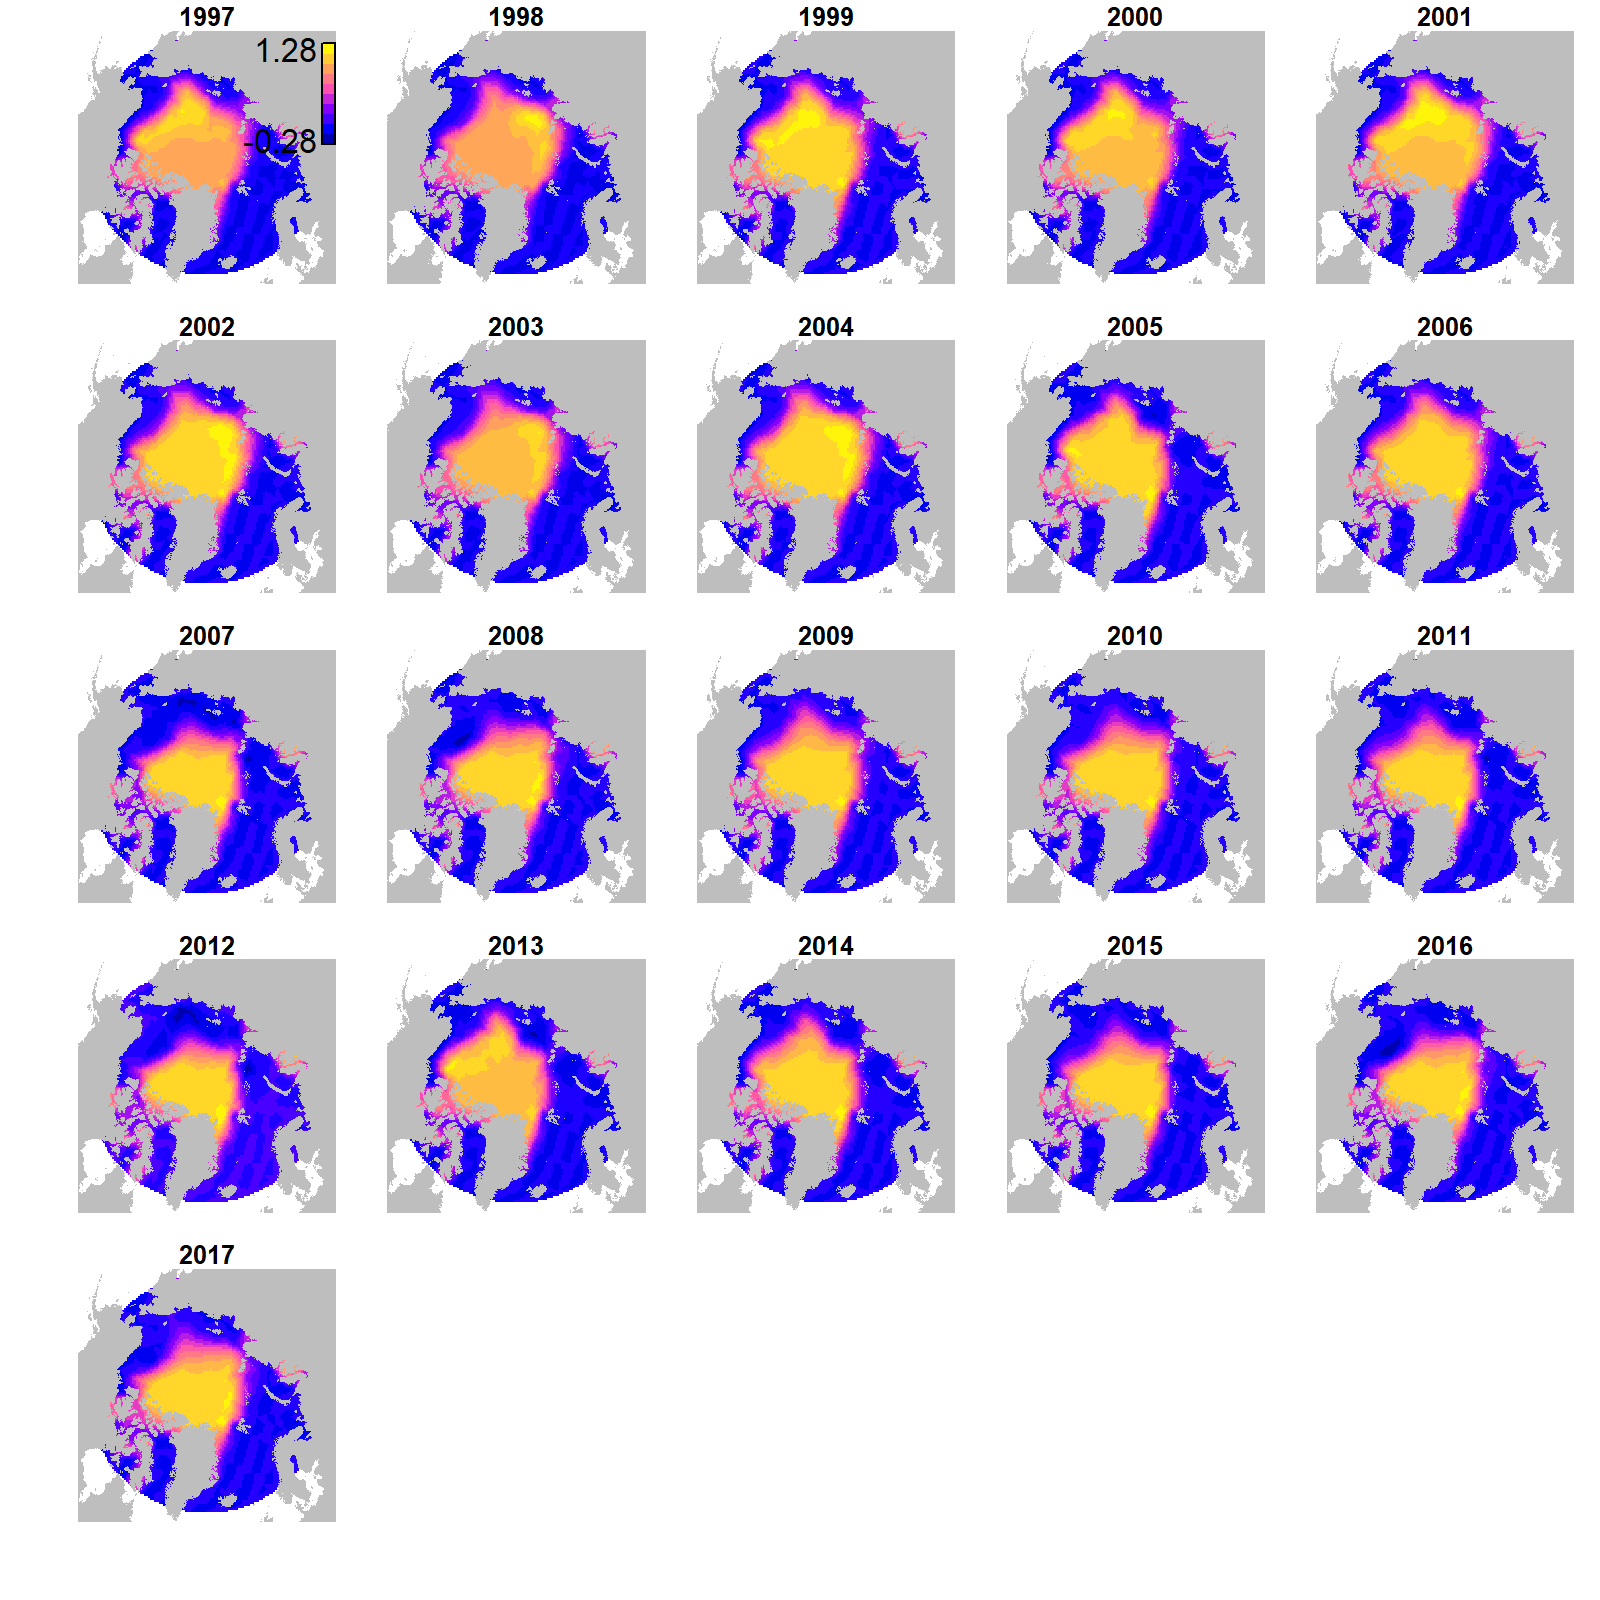
\includegraphics[width=5.5in]{Chap_9/sea_ice_full.png}
    \label{fig:Chap9_sea_ice_full}
\end{figure}

We first illustrate the usefulness of this EOF-GLLVM using a physical system that is undergoing rapid dynamics due to directional climate change as well as climate oscillations.  We specifically download sea-ice concentrations for the Arctic in September, which are available based on satellite observations \cite{comiso_trends_2008}.  We download data from 1997 to 2017 from PolarWatch\footnote{These data were provided by NOAA's Center for Satellite Applications \& Research (STAR) and the CoastWatch program and distributed by NOAA/NMFS/SWFSC/ERD.}, and then restrict data to within 3000 km of the north pole.  For illustration, we first fit the spatio-temporal index model (i.e., \( \Lambda = \sigma \mathbf{I} \)) using an identity link and normal distribution, and present results to visualize spatial and temporal patterns in sea ice over the past two decades.  Predicted summer sea-ice concentrations (Fig. \ref{fig:Chap9_sea_ice_full}) show notable declines in average fall extent from early years (1997--2000) to late years (2014--2017).  For example, a northern passage (resulting from ice-free waters north of Russia) seems feasible from 2011 to 2015.  However, the spatio-temporal index model does not itself estimate any parameters that can be directly interpreted to draw large-scale inference about dominant patterns; instead, it is helpful primarily to visualize the apparent decrease in sea-ice extent in the waters near Alaska and Russia.   

\begin{figure}[!ht]
    \caption[Comparison of estimated sea ice extent]{Predicted spatial extent of Sept. Arctic sea ice from the spatio-temporal index standardization model (Eq. \ref{eq:Chap8_spatiotemporal}) or the EOF model with two modes of variability (Eq. \ref{eq:Chap9_EOF}).}
    \centering
    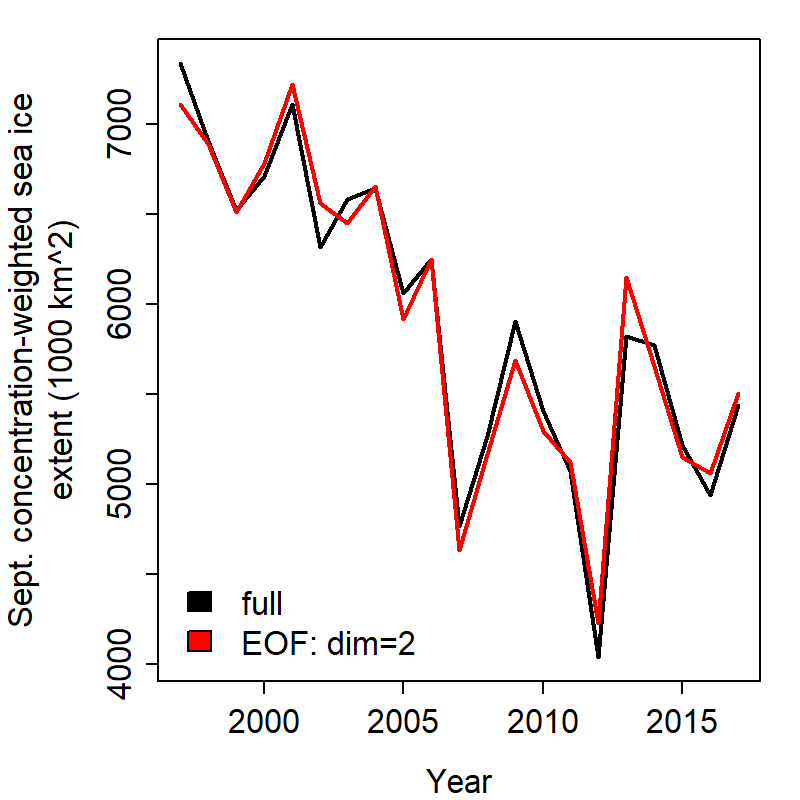
\includegraphics[width=4in]{Chap_9/sea_ice_extent.png}
    \label{fig:Chap9_sea_ice_extent}
\end{figure}

We then contrast these predictions with those arising from an EOF-GLLVM while estimating two modes of variability.  We specifically compare predictions of sea-ice area, calculated as the area-weighted sum of sea-ice concentrations from both the ``index standardization" and the EOF-GLLVM models.  This shows that both models estimate nearly identical trends and interannual variability, including estimates of low sea-ice extent in 2007 and 2012 (Fig. \ref{fig:Chap9_sea_ice_extent}).  We therefore conclude that the EOF-GLLVM is a suitable approximation for the full interannual dynamics of Arctic sea ice concentrations over this period, despite estimating considerably fewer random effects than the spatio-temporal index model.  

\begin{figure}[!ht]
    \caption[Empirical orthogonal function for Arctic sea ice concentrations]{Empirical orthogonal function model components that explain Arctic Sea ice concentrations (see Section \ref{eq:Chap9_EOF}), including the average spatial component (top-left panel), the spatial response for both models (top-right and bottom-left), and the temporal index associated with each mode (bottom-right).}
    \centering
    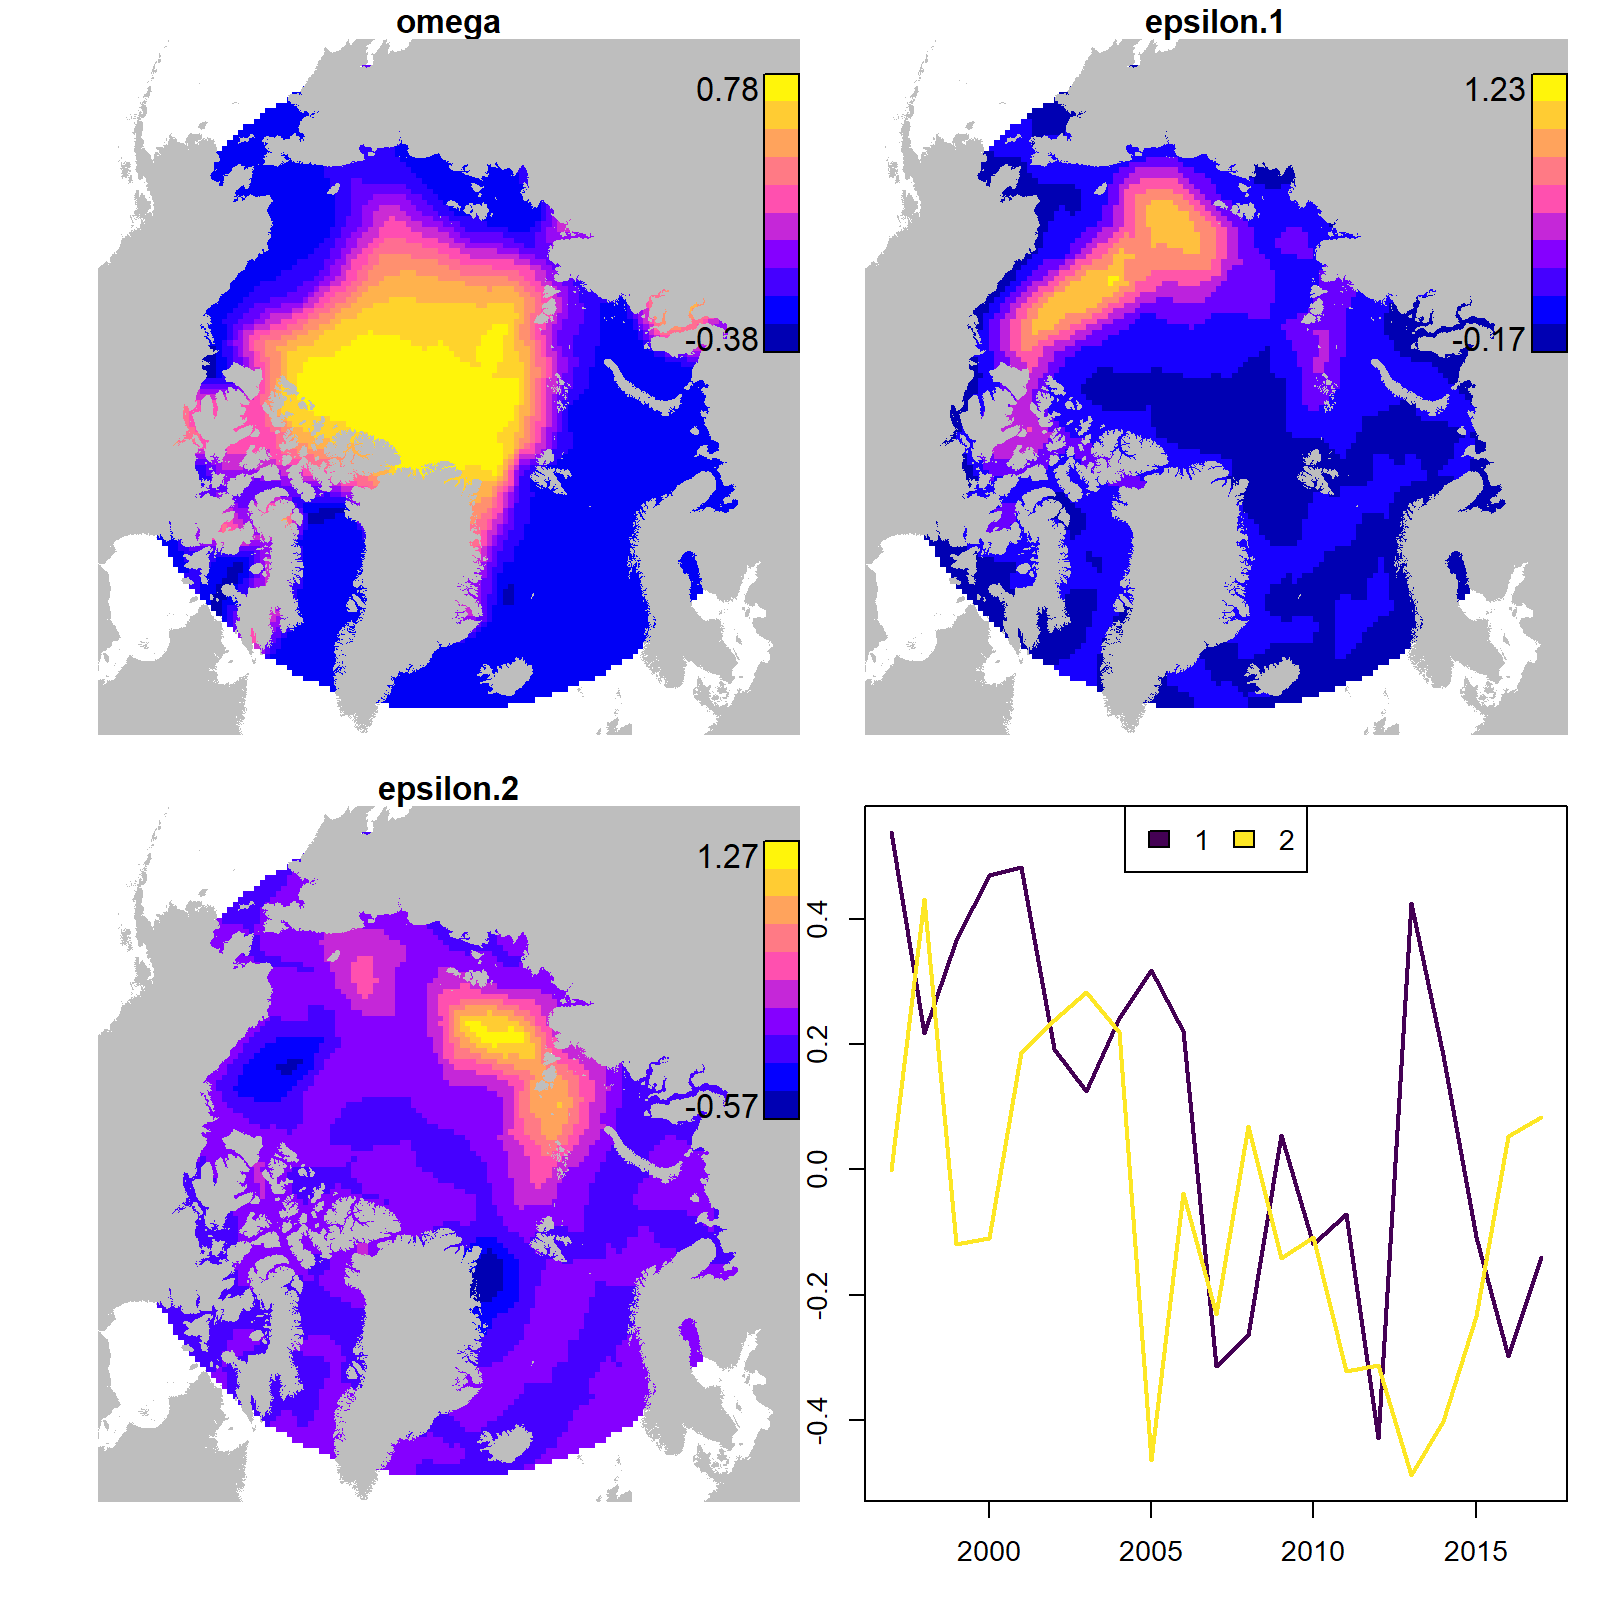
\includegraphics[width=5.5in]{Chap_9/EOF=2.png}
    \label{fig:Chap9_EOF=2}
\end{figure}

Given that the EOF model is a suitable approximation to the full spatio-temporal dynamics, we next proceed to visualize and interpret individual model components (Fig. \ref{fig:Chap9_EOF=2}).  As expected, the average spatial component \( \omega \) captures the multidecadal average concentration of sea ice, including consistently high concentrations from the north pole to Greenland and west to the Canadian Arctic archipelago. By contrast, the first mode of variability is associated with elevated sea-ice concentrations north of the Pacific gateway to the Arctic (i.e., poleward of Alaska and eastern Russia), while the second mode is associated with elevated sea-ice poleward from the Kara and Laptev Seas north of central Russia.  The first mode (purple line in bottom-right panel of Fig. \ref{fig:Chap9_EOF=2}) showed a precipitous decline 2006--2007 that persists over the following years (with a notable exception of 2013--2014), while the second mode (yellow line in bottom-right panel) showed more consistency over time with the exception of a decline and subsequent recovery from 2010 to 2016.  From this dimension-reduction exercise, we therefore conclude that:
\begin{itemize}
    \item Two dominant modes of physical variability can explain synchronous changes in summer sea-ice concentration through the Arctic;

    \item The primary mode of variability represents progressive warming in the Pacific gateway to the Arctic; and

    \item The secondary mode represents fluctuations and a slower decline in the Kara and Laptev seas that might enable a northern passage across Russian waters.
\end{itemize}
These dynamics are much more clearly visualized using EOF (Fig. \ref{fig:Chap9_EOF=2}) than inspecting maps of sea-ice concentration arising from the index-standardization model (Fig. \ref{fig:Chap9_sea_ice_full}), despite these two models resulting in essentially identical predictions of underlying dynamics.  

\section{Confirmatory Factor Analysis and Spatially Varying Coefficients} \label{sec:Chap9_confirmatory_factor_model}

In the preceding section, we summarized spatio-temporal dynamics using an EOF model.  This then represented physical teleconnections (synchronous dynamics at geographically distant locations) using ``modes of variability" that each include a time-series and response map.  Notably, we imposed no structure on the loadings matrix \( \Lambda \) representing the association of each year with each mode.  This unstructured loadings matrix also arose in Section \ref{sec:Chap4_factor_model}, where it was called a ``factor analysis" model.  Using an unstructured loadings matrix for factor analysis is also sometimes called \myindex{exploratory factor analysis}.  

As alternative to exploratory factor analysis, we next introduce \myindex{confirmatory factor analysis}.  As their names imply, exploratory and confirmatory factor models can be used iteratively to identify and then attribute observed variation to hypothesized ecological processes \cite{gruss_synthesis_2021,von_hardenberg_disentangling_2013}, including physical and ecological teleconnections.  To do so, we here replace the unstructured loadings matrix (Eq. \ref{eq:Chap4_loadings_matrix}) with one or more columns containing known values or constraints.  For example, we might specify that loadings matrix \( \Lambda \) has a single column containing a time-series that is hypothesized to drive synchronous variation in a target variable.  

To demonstrate, we expand the case study for Alaska pollock that was previously used to introduce interannual variation in spatio-temporal models (Section \ref{sec:Chap8_interannual_dynamics}). We specifically expand Eq. \ref{eq:Chap8_spatiotemporal} by adding a spatially varying response to a time-series measuring the spatial extent of cold waters near the seafloor (termed ``cold pool extent" and introduced in Section \ref{sec:Chap8_changes_in_spatial_distribution}): 

\begin{equation}
\begin{gathered} \label{eq:Chap9_confirmatory_factor_model}
  \mathrm{log}( d_{s,t} ) = \beta_t + \omega_s + \epsilon_{s,t} + x_t \xi_s \\
  \mathbf{\omega} \sim \mathrm{MVN}( \mathbf{0, \Sigma}_{\omega} ) \\
  \mathbf{\epsilon}_t \sim \mathrm{MVN}( \mathbf{0, \Sigma}_{\epsilon} ) \\
  \mathbf{\xi} \sim \mathrm{MVN}( \mathbf{0, \Sigma}_{\xi} ) 
\end{gathered}
\end{equation}
where \( x_t \) is now replacing a column of the exploratory factor-analysis model with a time series measuring an hypothesized mechanistic driver of spatio-temporal dynamics.  

In contrast to exploratory factor analysis, we can use confirmatory factor analysis to attribute large-scale patterns to a known covariate that is assumed to be exogenous (see Section \ref{sec:Chap7} for a discussion of exogeneity and attribution).  In this case, we visualize the expected changes in population density that are attributed to geophysical processes that are associated with cold-pool extent.  Examining the cold-pool response map for pollock (Fig. \ref{fig:Chap9_SVC_response}) shows that a larger-than-average cold-pool extent is associated with lower pollock densities in the waters south of St. Lawrence Island (i.e., essentially in the northwestern portion of the model domain), and elevated densities along the southwestern border of the survey area.  Given the lower frequency of sampling in the northern Bering Sea, it is unsurprising that the response map in these northern areas is estimated with greater uncertainty (right panel of Fig. \ref{fig:Chap9_SVC_response}).  In this specific application, decreased pollock densities south of St. Lawrence Island occurring in summers with a large cold pool is typically explained by noting that adult pollock migrate to avoid near freezing waters, and that the cold-pool arises mainly in those impacted areas.  

\begin{figure}[!ht]
    \caption[Pollock response to cold-pool extent]{Illustrating confirmatory factor analysis by replacing a mode of variability in an exploratory factor analysis model with a time series covariate.  In this case, we show the biomass-response associated with cold-pool extent for Alaska pollock.}
    \centering
    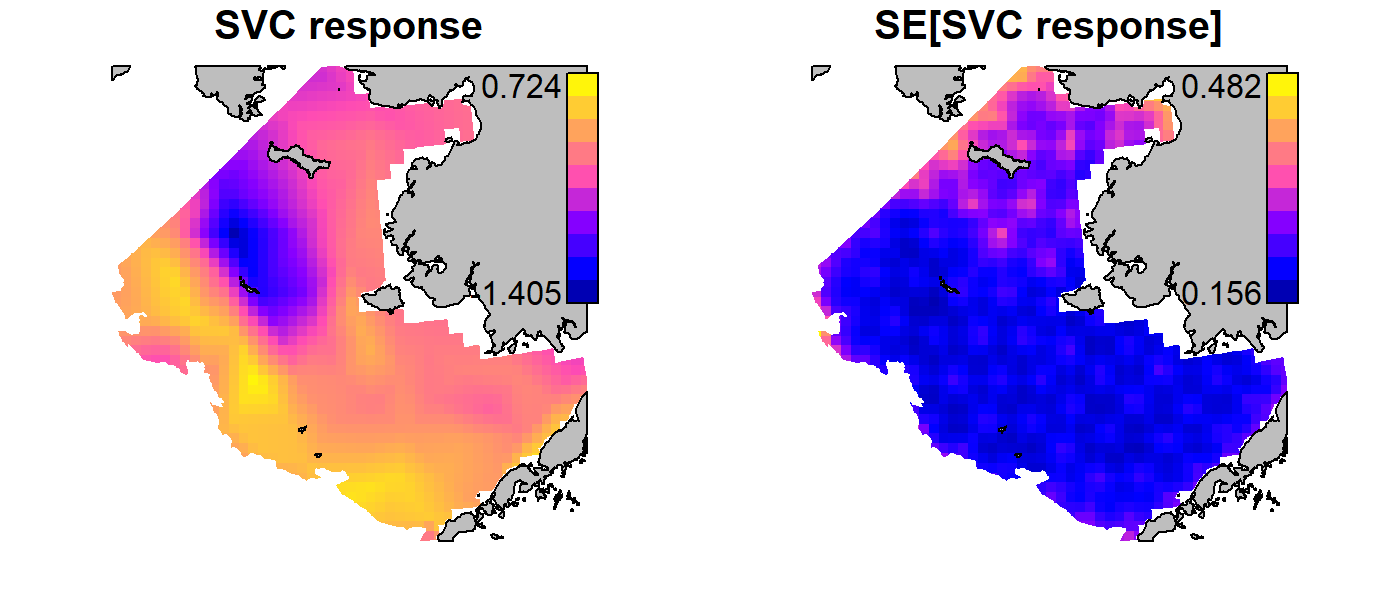
\includegraphics[width=5.5in]{Chap_9/SVC_response.png}
    \label{fig:Chap9_SVC_response}
\end{figure}

An analyst may also wonder about the potential that a spatial response like this could arise by chance.  To assess the ``statistical significance" of this confirmatory factor analysis, we could use a variety of statistical comparisons and diagnostics including using a likelihood-ratio test or the Akaike Information Criterion \cite{akaike_new_1974} to compare models with or without the spatially varying response.  However, for illustration, we here refit the same model while randomizing the order of the cold-pool index (i.e., sampling without replacement from \(x_t\)).  This randomized index is expected to have no remaining information about the dynamics of pollock, so we expect that a well-performing model will tend to estimate that it has a negligible impact.  As expected, this experiment results in an estimated standard deviation for the spatially varying response that approaches zero (Fig. \ref{fig:Chap9_SVC_response_randomized}).  This therefore confirms that including an uninformative index in a confirmatory factor-analysis model will tend to be eliminated from the model due to the shrinkage that occurs when estimating the variance of random effects.    

\begin{figure}[!ht]
    \caption[Pollock response to a randomized time-series]{Illustrating confirmatory factor analysis when replacing the cold-pool index with a randomized time-series, where the response (left-hand-side) uses a colorbar from --0.1 to 0.1 rather than the miniscule range of the estimated response.}
    \centering
    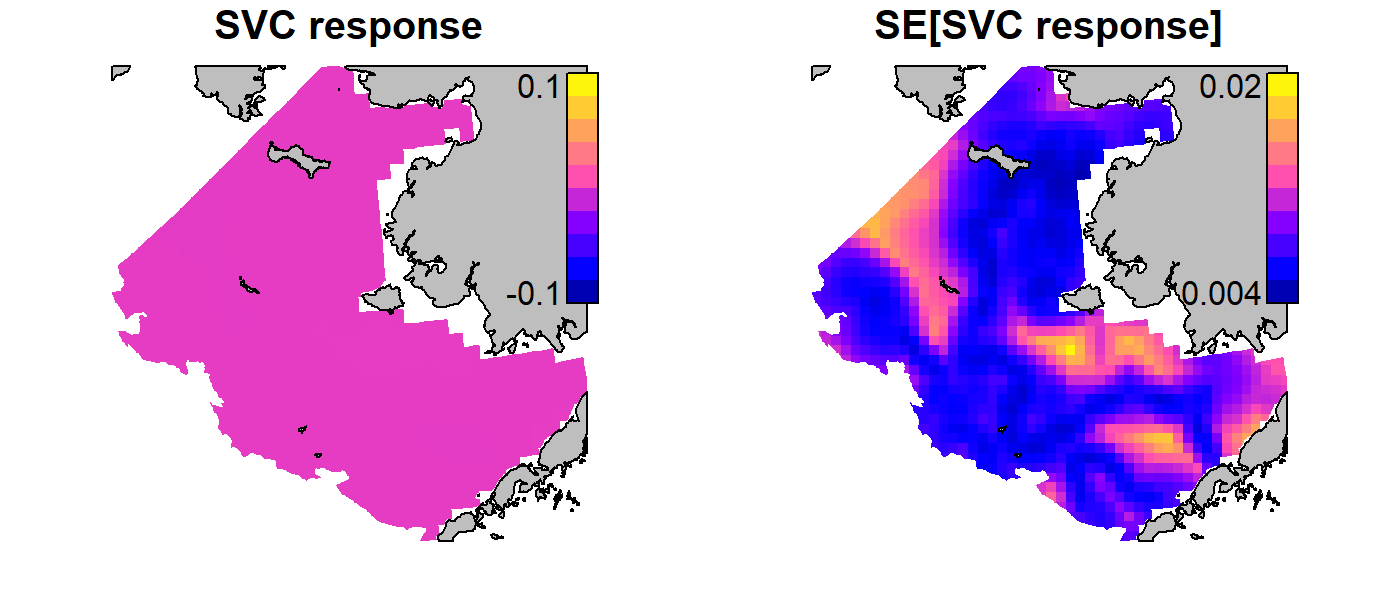
\includegraphics[width=5.5in]{Chap_9/SVC_response_randomized.png}
    \label{fig:Chap9_SVC_response_randomized}
\end{figure}

Beyond introducing the distinction between exploratory and confirmatory factor analysis, this example illustrates that a single regional index (cold-pool extent) can result in synchronous variation at multiple locations that are separated by large geographical distances.  These types of ecological teleconnections are likely ubiquitous in ecological systems, but are not well represented by predicting local densities solely based on local environmental conditions.  

\section{Chapter Summary}

In summary, we have showed that:
\begin{enumerate}
    \item Teleconnections (i.e., synchrony in dynamics for geographically distant locations) occur in many physical systems. Teleconnections occurring in physical drivers as well as ecological and evolutionary dynamics can given rise to ecological teleconnections, and these are dramatic and important in many ecosystems;

    \item Teleconnections can be identified by fitting an empirical orthogonal function (EOF) model.  EOF is conventionally estimated by fitting a principal components analysis to system measurements, but this definition has many drawbacks when applied to zero-inflated and right-skewed data from sampling designs that arise in ecology;
    
    \item This conventional PCA analysis for EOF can be extended by fitting a generalized linear latent variable model (EOF-GLLVM).  This involves estimating one or more time-series indices, where each index is associated with an estimated map of responses.  Applying a ``PCA rotation" to indices from an EOF-GLLVM then results in estimates that are directly comparable with PCA analysis;    
    
    \item In some cases, the EOF model can generate estimates of system dynamics that are similar to an unstructured spatio-temporal model.  In these cases, the EOF model provides a ``rank-reduced" and easy-to-interpret summary of system dynamics, while also estimating model components (e.g., average spatial patterns) that are typically excluded by the PCA analysis;

    \item EOF can be interpreted as one type of \textit{exploratory factor analysis}, and can be applied iteratively with \textit{confirmatory factor analysis} to attribute modes of variability to hypothesized drivers.  Specifically, confirmatory factor analysis can be applied by replacing an estimated EOF index with a known time-series that is then fitted with a spatially varying response.  Iterating between exploratory and confirmatory factor models allows us to visualize dominant spatio-temporal patterns without any constraints (exploratory models), and then to see what portion of these patterns can be explained by hypothesized regional conditions (confirmatory models).
\end{enumerate}

\section{Exercise}

The EOF-GLLVM (Eq. \ref{eq:Chap9_GLLVM}) and the spatio-temporal index model (Eq. \ref{eq:Chap8_spatiotemporal}) both estimate spatio-temporal variation, and differ in how the spatio-temporal term \(\mathbf{\Epsilon}\) is specified.  Please fit the spatio-temporal index model to spatially balanced data (i.e., Arctic sea ice concentrations) and then apply the PCA algorithm for fitting EOF (Section \ref{sec:Chap9_EOF}) to the estimated densities.  How does this two-stage approach differ from results obtained when fitting the EOF-GLLVM directly and doing both stages jointly?  Now, please repeat the exercise while dropping data from a large portion of the spatial domain in every other year (i.e., using a spatially blocked cross-validation design \cite{roberts_cross-validation_2017}).  Are the differences in estimates between these two approaches greater when analyzing spatially unbalanced data?    

